\section{Introducing SPIND}

We will now discuss our proposed algorithm $SPIND$, which stands for \textbf{s}calable \textbf{p}artial \textbf{in}clusion \textbf{d}ependencies. Further the german word $Spind$ is a special kind of closet and often multiple "Spinds" are placed next to each other. This is a metaphor to the algorithms procedure. Every input relation will be transformed to a "Spind" of sorted values with connected attributes (attribute combinations), which is surely bigger than a $BINDER$ bucket, but there are far fewer "Spinds" than $BINDER$ would create buckets.

\begin{figure}[h]
    \centering
    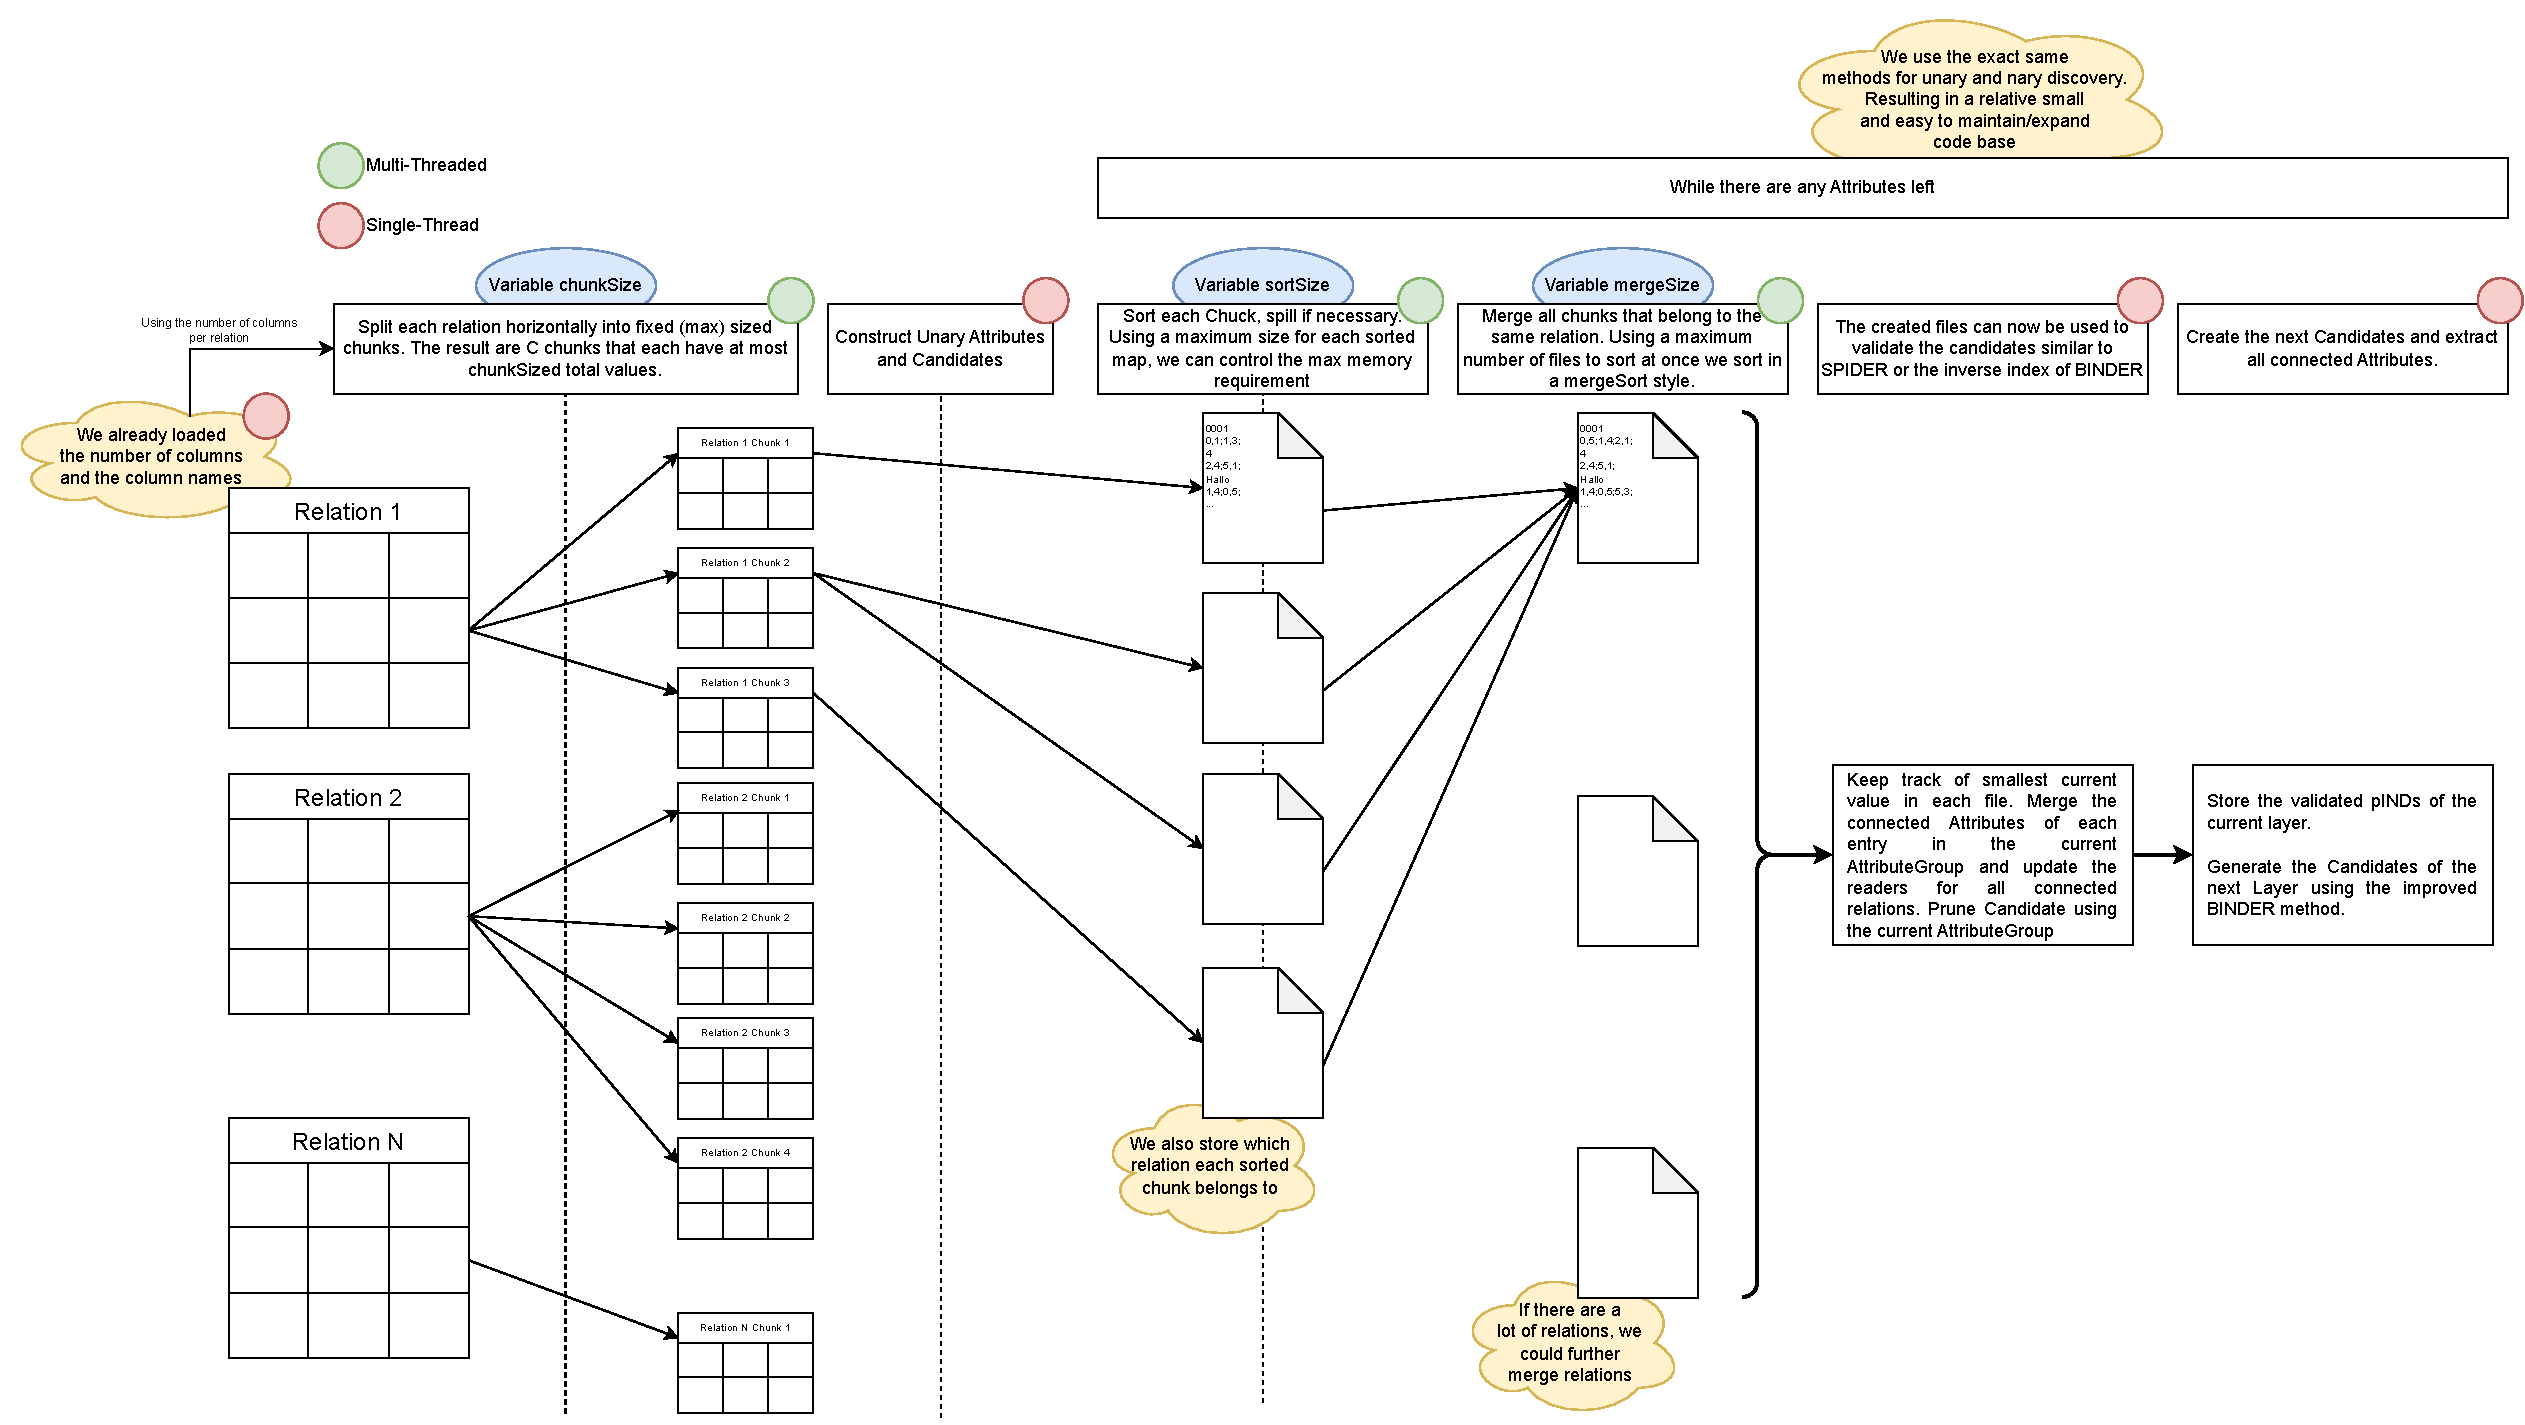
\includegraphics[width=0.99\textwidth]{files/SPIND.pdf}
    \caption{Conceptual overview of \textit{SPIND}}
    \label{fig:spind}
\end{figure}

\subsection{Chunking the input relations}
Modern CPUs have multiple cores which can execute tasks in parallel. Most of the related work did not try to utilize multi-threading. $SPIND$ will multi-thread as many parts of the execution as possible to best utilize the available hardware. This goal requires us to find independent tasks which can be processes in parallel. \\

\noindent The execution starts by fetching some very basic information about the input relations. For each relational instance (input table) $SPIND$ will extract the header column (if present) and store the number of columns each table has. Using a constant $CHUNK\_SIZE$ which is set by the user, we spilt each relation into somewhat equal parts. Each chunk will consist of at most $\lfloor \frac{CHUNK\_SIZE}{\# cloumns \: in \: relation} \rfloor$ rows. The complexity of processing a relation directly depends on the number of total values in that relation. While this may be an oversimplification since there are many more factors, like the distribution of duplicate values, the raw size is easy to modify and a heuristic that can be applied without any specific dataset knowledge. Each of the resulting chunks is associated with exactly one relation and carries a subset of that relations rows. \\

\noindent Chunking is done exactly once at the very start and is not repeated for n-ary layers. We reuse the same chunks in every layer of the n-ary pIND discovery. \\

\noindent Since $SPIND$ almost always operates on the relation layer, a hash based partitioning, similar to $BINDER$, is not feasible. For the validation, we need to descend to the attribute layer and there we need to know which attributes share some values. A partitioning would therefore be required to split the dataset into $n$ groups $G_1, \dots, G_n$ such that if $row_i \in G_j$ than 
\begin{itemize}
    \item[1)] $\forall \: row_k \in G \setminus G_j : row_i \cap row_k = \emptyset$
    \item[2)] $row_i \cap row_k \not = \emptyset \: \forall row_k \in G_j$
\end{itemize}
To find such groups we would need knowledge of all values in a relation. Even if we expand the groups row by row and merge when necessary, solving this grouping problem would create a lot of new complexity. To still understand the potential benefit, table 

\begin{center}
    \begin{tabular}{c|c|c|c|c} 
     dataset & average & median & min & max\\ 
     \hline\hline
     data.gov & - & - & - & -\\ 
     \hline
     musicbrainz & - & - & - & -\\
    \end{tabular}
\end{center}

\subsection{Sorting Chunks}
Once the chunks are created we want to sort each of them. Sorting is needed for the later validation. Every chunk is processed in the same way and processing is executed in parallel. We attach a $CSVReader$ to a chuck and provide the information, which attributes (attribute combinations) are relevant. Assume we are in the third layer and the only candidates which are connected with the relation of the chuck are the column combination $[1, 2, 3]$ and the column combination $[4, 5, 1]$. We would pass these relevant combinations as a list. Now the chuck is processed line by line, where we update the connected attributes to their current value after the line is read. We update a map which maps present values to the attributes which carry them, including the number of occurrences. This results in a two layer map. First the value is mapped to the connected attributes and then the connected attribute is mapped to the occurrences. Eventually this process would overflow the available main memory. Therefor we limit the size of the map by a constant called $SORT\_SIZE$. Once the map size reaches this constant or we finished sorting, we need to save the values to disk. First, the key set of the outer map is sorted by the included values. Afterwards we iterate over the sorted keys and persist each entry by first writing a line containing the value and then a line containing the persisted attributes. The attributes are persisted in the pattern $"attributeId_1,occurrences_1;attributeId_2,occurrences_2;...;"$. Figure \ref{fig:sorting} offers an illustration of this process. Persisting the connected attributes like that enables efficient merging of chunks later. For every file that is created, we store the path of the sorted (sub) chunk and in the end return that list.

\begin{figure}[h]
    \centering
    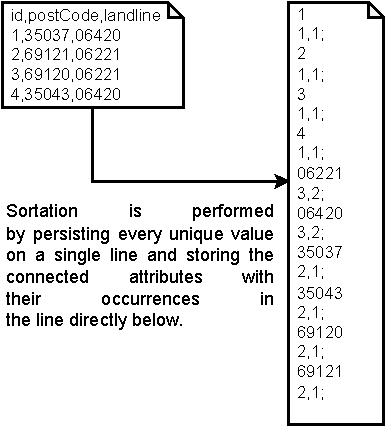
\includegraphics[width=0.45\textwidth]{files/Sorting.pdf}
    \caption{Simplified illustration of the sorting process.}
    \label{fig:sorting}
\end{figure}

\subsection{Merging (spilled) Chunks}
We now have a bunch of files which are all sorted by themselves. The next step is to merge all the files with originated from the same relation. Again, this is computed in parallel. To avoid too many files being opened at the same time the constant $MERGE\_SIZE$ can be used to limit the number of files which are being sorted per thread. Due to multithreading the actual number of simultaneously opened files is $\#threads \cdot (MERGE\_SIZE + 1)$. The plus one originates since we always need to open the resulting output file of a merge as well.
% TODO decide on default and perform experiments


\subsection{Validation}